\documentclass[tikz,10pt,oneside,a4paper]{report}

% \usepackage[utf8]{inputenc} % specify input encoding, this should match the encoding of your editor
% \usepackage[]{fontenc}	    % specify the output encoding of PDF file.
\usepackage[english]{babel} % hyphenation patterns

% \usepackage{syntonly}
\usepackage{amsmath, amsthm, amssymb}
\usepackage{xiunitx}	% provide commands for various SI units
\usepackage{bm}	% bold math
\usepackage{enumitem}	% style of list item
\usepackage{fancyhdr}	% set header and footer
\usepackage{float}	% provide the placement option 'H', enforcing the placement exactly at that point of floating env.
%    \pagestyle{fancy}
\usepackage[colorlinks]{hyperref}   % make colored hyperlink
    \hypersetup{
	colorlinks = true,
	linkcolor = black,
	urlcolor = blue,
    }
\usepackage{listings}	% Code presentation
% \lstset{
%     language = TeX,
%     backgroundcolor = \color{white},
%     basicstyle = \footnotesize,
%     breakatwhitespace = false,	% automatics breaks at whitespace
%     breaklines = true,		% automatics line break
%     captionpos = b,		% caption-position at bottom
%     commentstyle = \color{blue},
%     escapeinside = {\%*}{*)},	% 
%     identifierstyle=,		% nothing happen
%     keepsapces = true,		% keep spaces in text
%     keywordstyle = \color{brown},
%     numbers = none,		% line numbers
%     numbersep = 5pt,		% how far line-numbers away from code
%     numberstyle = \tiny\color{gray}
%     stepnumebr = 2,		% If this option is 1, then each line will be numbered
%     stringstyle = \color{cyan},	% string literal style
%     tablesize = 2,		
% }
\usepackage{makeidx}
\usepackage{makecell}	% line breaking in a table cell
\usepackage{multicol}	% multicolumns environment in a table
% \usepackage{tabbing}	% tabbing env.
\usepackage{tabularx}	% another table environment
\usepackage[dvipsnames]{xcolor}   % colored text
\usepackage{tikz}
    \usetikzlibrary{arrows,shapes,chains,positioning}
    \usetikzlibrary{decorations.markings}
% \usepackage{graphicx} % when used with tikz package, don't load
	% this one, otherwise it will be loaded twice, and causing errors.
\graphicspath{{figures/}}    % note the double {} here.
\usepackage{wrapfig}	% wrap figures with text

\usepackage{eso-pic}	% AddToShipoutPictureBG
\usepackage{geometry}	% set margin
    \geometry{left=2.5cm,right=2.5cm,top=2.5cm,bottom=2.5cm}  % margin
\usepackage{lipsum} % produce random text
% \lipsum[1-4]	% produce 4 paragraphs
\usepackage{tabularx}	% align cell of fixed width 
\usepackage[most]{tcolorbox}	% color box (background)
\tcbset{
%    frame code={},
%    center title,
    left=0pt,
    right=0pt,
    top=0pt,
    bottom=0pt,
    colback=gray!70,
    colframe=white,
%    width=\dimexpr\textwidth\relax,
%    enlarge left by=0mm,
%    boxsep=5pt,
%    arc=0pt, outer arc=0pt,
}

\newcommand{\TOC}{Table of Contents}
\newcommand{\rom}[1]{\expandafter\@slowromancap\romannumeral #1@}
\newcommand{\Rom}[1]{\uppercase\expandafter{\romannumeral #1\relax}}
\newcommand{\red}[1]{\textcolor{red}{#1}}
\newcommand{\green}[1]{\textcolor{green}{#1}}
\newcommand{\blue}[1]{\textcolor{blue}{#1}}

\newcommand{\package}[1]{\colorbox{gray!15!}{\textcolor{red}{\it{#1}}}}
% \newcommand{\package}[1]{\lstinline[language=TeX, backgroundcolor=\color{gray}, basicstyle=\ttfamily\color{red}]{#1}}
\newcommand{\option}[1]{\colorbox{gray!15!}{\textcolor{blue}{\it{#1}}}}
% \newcommand{\option}[1]{\lstinline[language=TeX, backgroundcolor=\color{gray}, basicstyle=\color{blue}]{#1}}
\newcommand{\command}{\lstinline[language=TeX, backgroundcolor=\color{gray}, basicstyle=\color{RawSienna}]}
% \newcommand{\error}{\lstinline[language=sh, backgroundcolor=\color{gray}, basicstyle=\bfseries]}
\newcommand{\error}[1]{\colorbox{gray!15!}{\textbf{#1}}}

% add a 'Go to TOC' button in every page
\newcommand\AtPageUpperRight[1]{\AtPageUpperLeft{
    \put(\LenToUnit{\paperwidth},\LenToUnit{-0.1\paperheight}){#1}}}
\AddToShipoutPictureBG{
    \AtPageUpperRight{\put(-60,0){\hyperref[toc]{TOC}}}
}

\title{Hello World}
\author{Weibin Zhang \\ \url{weibin.zhang@stonybrook.edu} \\ 
\url{personal url} }
\date{\today}

% \setlength\parindent{0pt}

\begin{document}
\maketitle

\begin{multicols}{2}
    \tableofcontents\label{toc}    % to make a clickable toc, need hyperref package.
\end{multicols}


TODO:
\begin{itemize}
    \item style for code, for little chunks of code, for large chunks of code and their output.
\end{itemize}
\section{Introduction}
This is a personal introduction to \G{}.
https://www.ge.infn.it/geant4/events/nss2003/geant4lectures.html

Event biasing (variance reduction) techniques:
\begin{itemize}
    \item Primary event biasing	\\
	Biasing primary events/particles in terms of type of event, momentum
	distribution. 
    \item Leading particle biasing \\
	Taking only the most energetic (or most important) secondary. \\
	Simulating of a full shower is an expensive calculation. Instread of
	generating a full shower, trace only the most energetic secondary.
	Other secondary particles are immediately killed befoer being
	stacked. In this way, it is convenient to roughly estimate, e.g. the
	thickness of a shielf. Of course, physical quantities such as energy
	are not conserved for each event.
    \item Physics based biasing \\
	Biasing secondary production in terms of particle type, momentum
	distribution, cross-section, etc.
    \item Geometry based biasing \\
	Importance weighting for volume/region. \\
	Duplication of sudden death of tracks.	\\
	Define importance for each geometrical region, duplicate a track
	with relative weight if it goes toward more important region.
	Russian-roulette in another direction.
	Scoring particle flux with weights.
    \item Forced interaction \\
	Force a particular interaction, e.g. within a volume.
\end{itemize}

\section{Basic}
Basic ideas and concepts in \G{}.

\begin{description}
    \item [Step]
	Sample NMFP (Number of Mean Free Path) by the \emph{material independent way}	$\Rightarrow$ Using the xsection in the material where the particle is currently in, converts NMFP to the PL (physical length) $\Rightarrow$ The process which has the minimum PL determines the step length.
\end{description}
\subsection{Example}
\begin{enumerate}
    \item General
	\begin{enumerate}
	    \item Configure the \textbf{Run}
	    \item Configure the \textbf{Event} Loop
	\end{enumerate}
    \item Experimental set-up
	\begin{enumerate}
	    \item geometrical set-up.
	    \item the coordinates of impact of tracks in the layers of the
		tracker, energy release in the strips of the tracker.
	    \item energy deposited in calorimeter
	    \item energy deposited in anticoincidence(?)
	    \item Digitise the hits, setting a threshold for the energy
		deposit in the tracker
	    \item Generate a trigger signal combining signals from different
		detectors.
	\end{enumerate}
    \item Physics
	\begin{enumerate}
	    \item Primary events
	    \item Electromagnetic processes appropriate to the energy range
		of the experiment
	    \item Hadronic processes
	\end{enumerate}
    \item Analysis
	\begin{enumerate}
	    \item x-y distribution of impact of the track
	    \item histograms during the simulation execution
	    \item store significant quantities in a ntuple
	    \item Plot energy distribution in the calorimeter
	\end{enumerate}
    \item Visualisation
	\begin{enumerate}
	    \item Visualize the experimental set-up
	    \item trakcs
	    \item hits
	\end{enumerate}
    \item UI
	\begin{enumerate}
	    \item Configure the tracker, by modifying the number of active
		planes, the pitch of the strips, the area of silicon tiles,
		the material of the converter.
	    \item Configure the calorimeter, by modifying the number of
		active elements, the number of layers.
	    \item Sources
	    \item Digisation by modifying threshold
	    \item Histograms
	\end{enumerate}
    \item Persistency
	\begin{enumerate}
	    \item Produce an intermediate output of the simulation at the
		level of hits in the tracker
	    \item Store significant results in FITS format
	    \item Read in an intermediate output for further elaboration.
	\end{enumerate}
\end{enumerate}

\chapter{Math}

%%%%%%%%%%%%%%%%%%%%%%%%%%%%%%%%%%%%%%%%%%%%%%%%%%%%%%%%%%%%%%%%%%%%%%%%
\section{Font}
Fonts in mathematical mode.
\begin{description}
    \item [\textbackslash{}mathit]  italic (default)
    \item [\textbackslash{}mathrm]  roman
	\[
	    \mathrm ABCDEFGHIJKLMNOPQRSTUVWXYZ
	    \]
	\verb|\rm|
	\[
	    \rm ABCDEFGHIJKLMNOPQRSTUVWXYZ
	    \]
    \item [\textbackslash{}mathbf]  bold
    \item [\textbackslash{}mathsf]  sans serif
	\[
	    \mathsf ABCDEFGHIJKLMNOPQRSTUVWXYZ
	    \]
	\verb|\sf|
	\[
	    \sf ABCDEFGHIJKLMNOPQRSTUVWXYZ
	    \]
    \item [\textbackslash{}mathtt]  typewritter
    \item [\textbackslash{}mathcal] calligraphic (upper case only)
	\[
	    \mathcal ABCDEFGHIJKLMNOPQRSTUVWXYZ
	    \]
	\verb|\cal|
	\[
	    \cal ABCDEFGHIJKLMNOPQRSTUVWXYZ
	    \]
\end{description}
The recommended way to obtain ordinary text in displayed mathematical 
formulae is to use \verb|\hbox|.
\[
    M^\bot = \{ f \in V' : f(m) = 0 \hbox{ for all } m \in M \}.
    \]
Note the space before and after 'for all' in the input.

\subsection{Space}
\begin{lstlisting}[language=TeX]
    \begin{equation*}
	\begin{aligned}
	    f(x) =& x^2\! + 3x\! + 2 \\
	    f(x) =& x^2 + 3x + 2 \\
	    f(x) =& x^2\, + 3x\, + 2 \\
	    f(x) =& x^2\: + 3x\: + 2 \\
	    f(x) =& x^2\; + 3x\; + 2 \\
	    f(x) =& x^2\ + 3x\ + 2 \\
	    f(x) =& x^2\quad + 3x\quad + 2 \\
	    f(x) =& x^2\qquad + 3x\qquad + 2 \\
	\end{aligned}
    \end{equation}
\end{lstlisting}

\begin{equation*}
    \begin{aligned}
	f(x) =& x^2\! + 3x\! + 2 \\
	f(x) =& x^2 + 3x + 2 \\
	f(x) =& x^2\, + 3x\, + 2 \\
	f(x) =& x^2\: + 3x\: + 2 \\
	f(x) =& x^2\; + 3x\; + 2 \\
	f(x) =& x^2\ + 3x\ + 2 \\
	f(x) =& x^2\quad + 3x\quad + 2 \\
	f(x) =& x^2\qquad + 3x\qquad + 2 \\
    \end{aligned}
\end{equation*}

%%%%%%%%%%%%%%%%%%%%%%%%%%%%%%%%%%%%%%%%%%%%%%%%%%%%%%%%%%%%%%%%%%%%%%%%
\section{Symbols}

%%%%%%%%%%%%%%%%%%%%%%%%%%%%%%%%%%%%%%%%%%%%%%%%
\subsection{Greek Letters}
\begin{table}[!htbp]
    \centering
    \begin{tabular}{lp{2cm}lp{2cm}}
	\verb|\epsilon|	& $\epsilon$	& \verb|\varepsilon|	& $\varepsilon$    \\
	\verb|\theta|	& $\theta$	& \verb|\vartheta|	& $\vartheta$   \\
	\verb|\pi|	& $\pi$		& \verb|\varpi|		& $\varpi$    \\
	\verb|\rho|	& $\rho$	& \verb|\varrho|	& $\varrho$    \\
	\verb|\sigma|	& $\sigma$	& \verb|\varsigma|	& $\varsigma$    \\
	\verb|\phi|	& $\phi$	& \verb|\varphi|	& $\varphi$    \\
	\hline
	\verb|\zeta|	& $\zeta$	& \verb|\iota|		& $\iota$    \\
	\verb|\kappa|	& $\kappa$	& \verb|\xi|		& $\xi$    \\
	\verb|o|	& $o$		& \verb|\upsilon|	& $\upsilon$    \\
	\verb|\chi|	& $\chi$	& \verb|\psi|		& $\psi$    \\
    \end{tabular}
\end{table}

\subsection{Uppercase Greek Letters}
\begin{table}[H]
    \centering 
    \begin{tabular}{lp{2cm}lp{2cm}lp{2cm}}
	\verb|\Gamma|	& $\Gamma$  &
	\verb|\Xi|	& $\Xi$  &
	\verb|\Phi|	& $\Phi$    \\
	\verb|\Delta|	& $\Delta$  &
	\verb|\Pi|	& $\Pi$  &
	\verb|\Psi|	& $\Psi$    \\
	\verb|\Theta|	& $\Theta$  &
	\verb|\Sigma|	& $\Sigma$  &
	\verb|\Omega|	& $\Omega$	\\
	\verb|\Lambda|	& $\Lambda$  &
	\verb|\Upsilon|	& $\Upsilon$  &
	&   \\
    \end{tabular}
\end{table}

\subsection{Miscellaneous Symbols}
\begin{table}[!htbp]
    \centering
    \begin{tabular}{lp{2cm}lp{2cm}lp{2cm}}
	\verb|\aleph|	& $\aleph$	&
	\verb|\prime|	& $\prime$	&
	\verb|\forall|	& $\forall$	    \\
	\verb|\hbar|	& $\hbar$	& 
	\verb|\emptyset|	& $\emptyset$	& 
	\verb|\exists|	& $\exists$	    \\ 
	\verb|\imath|	& $\imath$	& 
	\verb|\nabla|	& $\nabla$	&   
	\verb|\neg|	& $\neg$	    \\ 
	\verb|\jmath|	& $\jmath$	& 
	\verb|\surd|	& $\surd$	& 
	\verb|\flat|	& $\flat$	    \\ 
	\verb|\ell|	& $\ell$	& 
	\verb|\top|	& $\top$	& 
	\verb|\natural|	& $\natural$	    \\ 
	\verb|\wp|	& $\wp$	& 
	\verb|\bot|	& $\bot$	& 
	\verb|\sharp|	& $\sharp$	    \\ 
	\verb|\Re|	& $\Re$	& 
	\verb/\|/	& $\|$	& 
	\verb|\clubsuit|	& $\clubsuit$	    \\
	\verb|\Im|	& $\Im$	& 
	\verb|\angle|	& $\angle$	& 
	\verb|\diamondsuit|	& $\diamondsuit$    \\
	\verb|\partial|	& $\partial$	& 
	\verb|\triangle|	& $\triangle$	& 
	\verb|\heartsuit|	& $\heartsuit$	\\
	\verb|\infty|	& $\infty$	& 
	\verb|\backslash|	& $\backslash$	& 
	\verb|\spadesuit|	& $\spadesuit$	\\
    \end{tabular}
\end{table}
	
%%%%%%%%%%%%%%%%%%%%%%%%%%%%%%%%%%%%%%%%%%%%%%%%
\subsection{``Large" Operators}
\begin{table}[!htbp]
    \centering
    \begin{tabular}{lp{2cm}lp{2cm}lp{2cm}}
	\verb|\sum|	    & $\sum$	&
	\verb|\bigcap|	    & $\bigcap$	&
	\verb|\bigodot|	    & $\bigodot$	\\
	\verb|\prod|	    & $\prod$	&
	\verb|\bigcup|	    & $\bigcup$	&
	\verb|\bigotimes|   & $\bigotimes$	\\
	\verb|\coprod|	    & $\coprod$	&
	\verb|\bigsqcup|    & $\bigsqcup$	&
	\verb|\bigoplus|    & $\bigoplus$	\\
	\verb|\int|	    & $\int$	&
	\verb|\bigvee|	    & $\bigvee$	&
	\verb|\biguplus|    & $\biguplus$	\\
	\verb|\oint|	    & $\oint$	&
	\verb|\bigwedge|    & $\bigwedge$	&
	&   \\
    \end{tabular}
\end{table}


%%%%%%%%%%%%%%%%%%%%%%%%%%%%%%%%%%%%%%%%%%%%%%%%
\subsection{Binary Operators}
\begin{table}[H]
    \centering
    \begin{tabular}{lp{2cm}lp{2cm}lp{2cm}}
	\verb|\pm|	    & $\pm$	&
	\verb|\cap|	    & $\cap$	&
	\verb|\vee|	    & $\vee$	\\
	\verb|\mp|	    & $\mp$	&
	\verb|\cup|	    & $\cup$	&
	\verb|\wedge|	    & $\wedge$	\\
	\verb|\setminus|    & $\setminus$	&
	\verb|\uplus|	    & $\uplus$	&
	\verb|\oplus|	    & $\oplus$	\\
	\verb|\cdot|	    & $\cdot$	&
	\verb|\sqcap|	    & $\sqcap$	&
	\verb|\ominus|	    & $\ominus$	\\
	\verb|\times|	    & $\times$	&
	\verb|\sqcup|	    & $\sqcup$	&
	\verb|\ominus|	    & $\ominus$	\\
	\verb|\ast|	    & $\ast$	&
	\verb|\triangleleft|	    & $\triangleleft$	&
	\verb|\oslash|	    & $\oslash$	\\
	\verb|\star|	    & $\star$	&
	\verb|\triangleright|	    & $\triangleright$	&
	\verb|\odot|	    & $\odot$	\\
	\verb|\diamond|	    & $\diamond$	&
	\verb|\wr|	    & $\wr$	&
	\verb|\dagger|	    & $\dagger$	\\
	\verb|\circ|	    & $\circ$	&
	\verb|\bigcirc|	    & $\bigcirc$	&
	\verb|\ddagger|	    & $\ddagger$	\\
	\verb|\bullet|	    & $\bullet$	&
	\verb|\bigtriangleup|	    & $\bigtriangleup$	&
	\verb|\amalg|	    & $\amalg$	\\
	\verb|\div|	    & $\div$	&
	\verb|\bigtriangledown|	    & $\bigtriangledown$	&
	&   \\
    \end{tabular}
\end{table}
%%%%%%%%%%%%%%%%%%%%%%%%%%%%%%%%%%%%%%%%%%%%%%%%
\subsection{Standard Functions and Embedded Text}
\begin{table}[!htbp]
    \centering
    \begin{tabular}{lp{2cm}lp{2cm}lp{2cm}}
	\verb|\arccos|	& $\arccos$ &
	\verb|\arcsin|	& $\arcsin$ & 
	\verb|\arctan|	& $\arctan$	\\ 
	\verb|\arg|	& $\arg$    & 
	\verb|\cos|	& $\cos$    & 
	\verb|\cosh|	& $\cosh$	\\ 
	\verb|\cot|	& $\cot$    & 
	\verb|\csc|	& $\csc$    & 
	\verb|\deg|	& $\deg$	\\ 
	\verb|\det|	& $\det$    & 
	\verb|\exp|	& $\exp$    & 
	\verb|\gcd|	& $\gcd$	\\ 
	\verb|\hom|	& $\hom$    & 
	\verb|\inf|	& $\inf$    & 
	\verb|\ker|	& $\ker$	\\ 
	\verb|\lg|	& $\lg$	& 
	\verb|\lim|	& $\lim$    & 
	\verb|\liminf|	& $\liminf$	\\ 
	\verb|\limsup|  & $\limsup$ & 
	\verb|\ln|	& $\ln$	&   
	\verb|\log|	& $\log$	\\ 
	\verb|\max|	& $\max$    & 
	\verb|\min|	& $\min$    & 
	\verb|\Pr|	& $\Pr$		\\   
	\verb|\sec|	& $\sec$    & 
	\verb|\sin|	& $\sin$    & 
	\verb|\sinh|	& $\sinh$	\\ 
	\verb|\sup|	& $\sup$    & 
	\verb|\tan|	& $\tan$    & 
	\verb|\tanh|	& $\tanh$	\\
    \end{tabular}
\end{table}

%%%%%%%%%%%%%%%%%%%%%%%%%%%%%%%%%%%%%%%%%%%%%%%%
\subsection{Relations}
\begin{table}[!htbp]
    \centering
    \begin{tabular}{lp{2cm}lp{2cm}lp{2cm}}
	\verb|\leq|	& $\leq$ &
	\verb|\geq|	& $\geq$ & 
	\verb|\equiv|	& $\equiv$	\\ 
	\verb|\prec|	& $\prec$    & 
	\verb|\succ|	& $\succ$    & 
	\verb|\sim|	& $\sim$	\\ 
	\verb|\preceq|	& $\preceq$    & 
	\verb|\succeq|	& $\succeq$    & 
	\verb|\simeq|	& $\simeq$	\\ 
	\verb|\ll|	& $\ll$    & 
	\verb|\gg|	& $\gg$    & 
	\verb|\asymp|	& $\asymp$	\\ 
	\verb|\subset|	& $\subset$    & 
	\verb|\supset|	& $\supset$    & 
	\verb|\approx|	& $\approx$	\\ 
	\verb|\subseteq|	& $\subseteq$	& 
	\verb|\supseteq|	& $\supseteq$    & 
	\verb|\cong|	& $\cong$	\\ 
	\verb|\sqsubseteq|  & $\sqsubseteq$ & 
	\verb|\sqsupseteq|	& $\sqsupseteq$	&   
	\verb|\bowtie|	& $\bowtie$	\\ 
	\verb|\in|	& $\in$    & 
	\verb|\ni|	& $\ni$    & 
	\verb|\propto|	& $\propto$		\\   
	\verb|\vdash|	& $\vdash$    & 
	\verb|\dashv|	& $\dashv$    & 
	\verb|\models|	& $\models$	\\ 
	\verb|\smile|	& $\smile$    & 
	\verb|\mid|	& $\mid$    & 
	\verb|\doteq|	& $\doteq$	\\
	\verb|\frown|	& $\frown$    & 
	\verb|\parallel|	& $\parallel$    & 
	\verb|\perp|	& $\perp$	\\
    \end{tabular}
\end{table}

%%%%%%%%%%%%%%%%%%%%%%%%%%%%%%%%%%%%%%%%%%%%%%%%
\subsection{Negated Relations}
\begin{table}[!htbp]
    \centering
    \begin{tabular}{lp{2cm}lp{2cm}lp{2cm}}
	\verb|\not<|		& $\not<$ &
	\verb|\not>|		& $\not>$ & 
	\verb|\not=|		& $\not=$	\\ 
	\verb|\not\leq|		& $\not\leq$ &
	\verb|\not\geq|		& $\not\geq$ & 
	\verb|\not\equiv|	& $\not\equiv$	\\ 
	\verb|\not\prec|	& $\not\prec$    & 
	\verb|\not\succ|	& $\not\succ$    & 
	\verb|\not\sim|		& $\not\sim$	\\ 
	\verb|\not\preceq|	& $\not\preceq$    & 
	\verb|\not\succeq|	& $\not\succeq$    & 
	\verb|\not\simeq|	& $\not\simeq$	\\ 
	\verb|\not\subset|	& $\not\subset$    & 
	\verb|\not\supset|	& $\not\supset$    & 
	\verb|\not\approx|	& $\not\approx$	\\ 
	\verb|\not\subseteq|    & $\not\subseteq$	& 
	\verb|\not\supseteq|    & $\not\supseteq$    & 
	\verb|\not\cong|	& $\not\cong$	\\ 
	\verb|\not\sqsubseteq|  & $\not\sqsubseteq$ & 
	\verb|\not\sqsupseteq|  & $\not\sqsupseteq$	&   
	\verb|\not\asymp|	& $\not\asymp$	\\ 
    \end{tabular}
\end{table}

%%%%%%%%%%%%%%%%%%%%%%%%%%%%%%%%%%%%%%%%%%%%%%%%
\subsection{Arrows}
\begin{table}[H]
    \centering
    \begin{tabular}{lp{2cm}lp{2cm}lp{2cm}}
	\verb|\leftarrow|	& $\leftarrow$	&
	\verb|\longleftarrow|	& $\longleftarrow$	&
	\verb|\uparrow|		& $\uparrow$	    \\
	\verb|\Leftarrow|	& $\Leftarrow$	&
	\verb|\Longleftarrow|	& $\Longleftarrow$	&
	\verb|\Uparrow|		& $\Uparrow$	    \\
	\verb|\rightarrow|	& $\rightarrow$	&
	\verb|\longrightarrow|	& $\longrightarrow$	&
	\verb|\downarrow|	& $\downarrow$	    \\
	\verb|\Rightarrow|	& $\Rightarrow$	&
	\verb|\Longrightarrow|	& $\Longrightarrow$	&
	\verb|\Downarrow|	& $\Downarrow$	    \\
	\verb|\leftrightarrow|	& $\leftrightarrow$	&
	\verb|\longleftrightarrow|	& $\longleftrightarrow$	&
	\verb|\updownarrow|	& $\updownarrow$	    \\
	\verb|\Leftrightarrow|	& $\Leftrightarrow$	&
	\verb|\Longleftrightarrow|	& $\Longleftrightarrow$	&
	\verb|\Updownarrow|	& $\Updownarrow$	    \\
	\verb|\mapsto|		& $\mapsto$	&
	\verb|\longmapsto|	& $\longmapsto$	&
	\verb|\nearrow|		& $\nearrow$	    \\
	\verb|\hookleftarrow|	& $\hookleftarrow$	&
	\verb|\hookrightarrow|	& $\hookrightarrow$	&
	\verb|\searrow|		& $\searrow$	    \\
	\verb|\leftharpoonup|	& $\leftharpoonup$  &   
	\verb|\rightharpoonup|	& $\rightharpoonup$  &   
	\verb|\swarrow|		& $\swarrow$	    \\
	\verb|\leftharpoondown|	& $\leftharpoondown$  &   
	\verb|\rightharpoondown|	& $\rightharpoondown$  &   
	\verb|\nwarrow|		& $\nwarrow$	    \\
	\verb|\rightleftharpoons|	& $\rightleftharpoons$  &   
	&   &	&   \\
    \end{tabular}
\end{table}

%%%%%%%%%%%%%%%%%%%%%%%%%%%%%%%%%%%%%%%%%%%%%%%%
\subsection{Openings}
\begin{table}[!htbp]
    \centering
    \begin{tabular}{lp{2cm}lp{2cm}lp{2cm}}
	\verb|\lbrack|	& $\lbrack$ &
	\verb|\lfloor|	& $\lfloor$ &
	\verb|\lceil|	& $\lceil$  \\
	\verb|\lbrace|	& $\lbrace$ &
	\verb|\langle|	& $\langle$ &
	&   \\
    \end{tabular}
\end{table}

%%%%%%%%%%%%%%%%%%%%%%%%%%%%%%%%%%%%%%%%%%%%%%%%
\subsection{Closings}
\begin{table}[!htbp]
    \centering
    \begin{tabular}{lp{2cm}lp{2cm}lp{2cm}}
	\verb|\rbrack|	& $\rbrack$ &
	\verb|\rfloor|	& $\rfloor$ &
	\verb|\rceil|	& $\rceil$  \\
	\verb|\rbrace|	& $\rbrace$ &
	\verb|\rangle|	& $\rangle$ &
	&   \\
    \end{tabular}
\end{table}

%%%%%%%%%%%%%%%%%%%%%%%%%%%%%%%%%%%%%%%%%%%%%%%%
\subsection{Alternative to some symbols}
\begin{table}[H]
    \centering
    \begin{tabular}{lll}
	$\ne$	    & \verb|\rbrack| or \verb|\neq| & (\verb|\not=|)	\\
	$\le$	    & \verb|\le|    & (\verb|\leq|)	\\
	$\ge$	    & \verb|\ge|    & (\verb|\geq|)	\\
	$\{$	    & \verb|\{|	    & (\verb|\lbrace|)	\\
	$\}$	    & \verb|\}|	    & (\verb|\rbrace|)	\\
	$\to$	    & \verb|\to|    & (\verb|\rightarrow|)	\\
	$\gets$	    & \verb|\gets|  & (\verb|\leftarrow|)	\\
	$\owns$	    & \verb|\owns|  & (\verb|\ni|)	\\
	$\land$	    & \verb|\land|  & (\verb|\wedge|)	\\
	$\owns$	    & \verb|\owns|  & (\verb|\vee|)	\\
	$\lor$	    & \verb|\lor|   & (\verb|\neg|)	\\
	$\vert$	    & \verb|\vert|  & (|)	\\
	$\Vert$	    & \verb|\Vert|  & (\verb/\|/)	\\
	$\iff$	    & \verb|\iff|   & (\verb|\Longleftrightarrow|, but with extra space at each end)	\\
	$\colon$    & \verb|\colon| & (:, but with less space around it and less likelihood of a line break after it.)	\\
    \end{tabular}
\end{table}

%%%%%%%%%%%%%%%%%%%%%%%%%%%%%%%%%%%%%%%%%%%%%%%%
\subsection{Accent}
\begin{table}[!htbp]
    \centering
    \begin{tabular}{ll}
	{\bf Command}	    & {\bf Accent}    \\
	\verb|\underline{a}|	& $\underline{a}$  \\
	\verb|\overline{a}|	& $\overline{a}$  \\
	\verb|\hat{a}|		& $\hat{a}$  \\
	\verb|\check{a}|	& $\check{a}$  \\
	\verb|\tilde{a}|	& $\tilde{a}$  \\
	\verb|\acute{a}|	& $\acute{a}$  \\
	\verb|\grave{a}|	& $\grave{a}$  \\
	\verb|\dot{a}|		& $\dot{a}$  \\
	\verb|\ddot{a}|		& $\ddot{a}$  \\
	\verb|\breve{a}|	& $\breve{a}$  \\
	\verb|\bar{a}|		& $\bar{a}$  \\
	\verb|\vec{a}|		& $\vec{a}$  \\
    \end{tabular}
\end{table}
You should bear in mind that when a character is underlined in a mathematical
manuscript, then it is normally typeset in bold face without any underlining. Underlining is used very rarely in print.

%%%%%%%%%%%%%%%%%%%%%%%%%%%%%%%%%%%%%%%%%%%%%%%%
\subsection{Other Physical and Mathematical Symbols}
\begin{table}[!htbp]
    \centering
    \begin{tabular}{lp{2cm}lp{2cm}}
	\verb|\binom{n}{k}| & $\binom{n}{k}$	&   &	\\
    \end{tabular}
\end{table}

\newpage
%%%%%%%%%%%%%%%%%%%%%%%%%%%%%%%%%%%%%%%%%%%%%%%%%%%%%%%%%%%%%%%%%%%%%%%%
\section{Matrix}
\subsection{pmatrix}
\[
    \sigma^{0} =
    \begin{pmatrix}
	1   & 0	\\
	0   & 1
    \end{pmatrix}
\]
\subsection{vmatrix}
\[
    \sigma^{0} =
    \begin{vmatrix}
	1   & 0	\\
	0   & 1
    \end{vmatrix}
\]
\subsection{bmatrix}
\[ \sigma^{0} =
    \begin{bmatrix}
	1   & 0	\\
	0   & 1
    \end{bmatrix}
\]
\subsection{aligned}
\begin{equation*}
    \left.  % \left and \right should match, but the delimiters need not to.
    \begin{aligned}
	u_x & = v_y \\
	u_y & = -v_x
    \end{aligned}
    \right\} \quad \text{Cauchy-Riemann Equations}
\end{equation*}
Spacing in math mode:
\begin{lstlisting}[language=TeX]
\quad,
\end{lstlisting}

%%%%%%%%%%%%%%%%%%%%%%%%%%%%%%%%%%%%%%%%%%%%%%%%%%%%%%%%%%%%%%%%%%%%%%%%
\section{cases}
\[
    |x| = 
    \begin{cases}
	x	&if\ x \geq 0	\cr
	-x	&if\ x < 0	\cr
    \end{cases}
    \]

%%%%%%%%%%%%%%%%%%%%%%%%%%%%%%%%%%%%%%%%%%%%%%%%%%%%%%%%%%%%%%%%%%%%%%%%
\section{Example}

\subsection{Integral}
\[
    \int_0^{+\infty} x^n e^{-x}\,dx = n!
    \]
Note the extra space before the $d$, which is produce by \verb|\,|.
Compare to case without \verb|\,|:
\[
    \int_0^{+\infty} x^n e^{-x} dx = n!
    \]

\[
    \int_0^1 \! \int_0^1 x^2 y^2 \,dx\,dy
    \]
In multiple integral, use \verb|\!| to remove a thin strip of unwanted space
to improve the appearance. Compare to case without \verb|\!|:
\[
    \int_0^1 \int_0^1 x^2 y^2 \,dx\,dy
    \]

% \usepackage{tikz}

% \begin{tikzpicture}[
%     font=\sffamily,
%     every matrix/.style={ampersand replacement=\&,column sep=2cm, row sep=2cm},
%     source/.style={draw, thick, rounded corners, fill=yellow!20, inner sep=.3cm},
%     process/.style={draw, thick, cirlce, fill=blue!20},
%     sink/.style={source, fill=green!20},
%     dots/.style={gray, scale=2},
%     to/.style={->,>=stealth',shorten >= 1pt, semithick, font=\sffamily\footnotesize},
%     every node/.style={align=center}
% ]
%     \matrix{
%         \node[]}
% \end{tikzpicture}


\chapter{Tikz}
This section introduce how to use tika package to produce wanted plots.

%%%%%%%%%%%%%%%%%%%%%%%%%%%%%%%%%%%%%%%%%%%%%%%%
\subsection{Simple shapes}

%%%%%%%%%%%%%%%%%%%%%%%%
\subsubsection{coordinate}
Coordinates can be specified in round brackets in an arbitrary TEX 
dimension either using Cartesion coordinates (comma separated), e.g. 
1cm in the x direction and 2pt in the y direction
\begin{tcolorbox}
\textsc{1cm, 2pt}
\end{tcolorbox}
\tikz\draw (0,0)--(0,2)--(2,0)--(0,0);


%%%%%%%%%%%%%%%%%%%%%%%%
\subsubsection{circle and ellipse}
\tikz\draw[line width=2mm, color=black] (0,0) circle (4ex);
\tikz\draw[fill=gray!30!white](0,0) ellipse (20pt and 28pt);
\tikz\draw[fill=gray!60!white] (0,0) ellipse (28pt and 20pt);

%%%%%%%%%%%%%%%%%%%%%%%%
\subsubsection{rectangle}
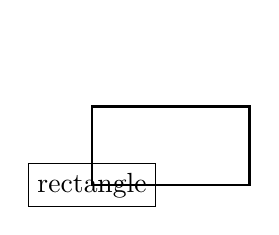
\begin{tikzpicture}
    \coordinate (O) (2,2);
    \node[draw, rectangle] (rec) at (0,0) {rectangle};	% here the coordinate (0,0) is the bottom left point's coor.
    \draw[thick] (O) rectangle ++(2,1);
\end{tikzpicture}
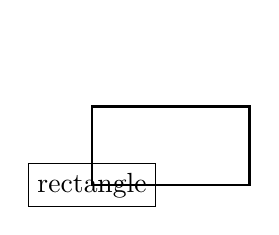
\begin{tikzpicture}
    \coordinate (O) (2,2);
    \node[draw, rectangle] (rec) at (0,0) {rectangle};	
    \draw[thick] (O) rectangle (2,1);
\end{tikzpicture}
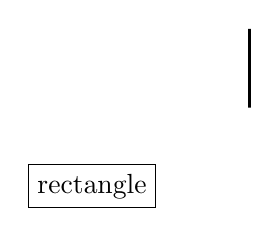
\begin{tikzpicture}
    \node[draw, rectangle] (rec) at (0,0) {rectangle};	
    \draw[thick] (2,2) rectangle (2,1);
\end{tikzpicture}
\begin{tikzpicture}
    \node[draw, rectangle] (rec) at (0,0) {rectangle};	
    \draw[thick] (2,2) rectangle ++(2,1);
\end{tikzpicture}
The \emph{rectangle} command requires the absolute corner coords. 
You are giving the increments in the second coordinates. So we can see
in the third above plot, it looks like a line, because the second coordinate
is not given as increments.

%%%%%%%%%%%%%%%%%%%%%%%%
\subsubsection{grid}
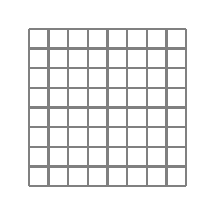
\begin{tikzpicture}
    \draw[step=0.25cm,gray,thick](-1,-1) grid(1,1);
\end{tikzpicture}

%%%%%%%%%%%%%%%%%%%%%%%%
\subsubsection{parabola, sin, cos}
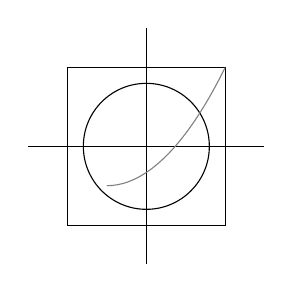
\begin{tikzpicture}
    \draw (-1.5, 0) -- (1.5, 0);
    \draw (0, -1.5) -- (0, 1.5);
    \draw (0, 0) circle (.8cm);
    \draw (-1, -1) rectangle (1, 1);
    \draw[gray] (-.5, -.5) parabola (1, 1);
\end{tikzpicture}
\tikz\draw[x=5pt, y=5pt] (0,0) parabola bend (4,16) (6,12);

{\bf sin} and {\bf cos} add a sine or cosine curve in the interval 
[0, $\pi/2$] such that the previous current point is at the start of the
curve and the curve ends at the given end point following it.

\tikz\draw[x=10pt,y=10pt] (0,0) sin (1,1) cos (2,0) sin (3,-1) cos (4,0)
			  (0,1) cos (1,0) sin (2,-1) cos (3,0) sin (4,1);
%%%%%%%%%%%%%%%%%%%%%%%%
\subsubsection{arc}
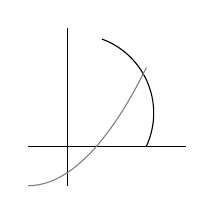
\begin{tikzpicture}
    \draw (-.5, 0) -- (1.5, 0);
    \draw (0, -.5) -- (0, 1.5);
    \draw (1, 0) arc (-25:70:1cm);
    \draw[gray] (-.5, -.5) parabola (1, 1);
\end{tikzpicture}
\hfill
\tikz\draw (0,0) arc (0:180:1cm);
\hfill
\hfill
\tikz\draw[fill=gray!50] (4, 0) -- +(30:1cm) arc (30:60:1cm) -- cycle;
\hfill
\tikz\draw[fill=gray!50] (4, 0) -- +(30:2cm) arc (30:60:1cm) -- cycle;

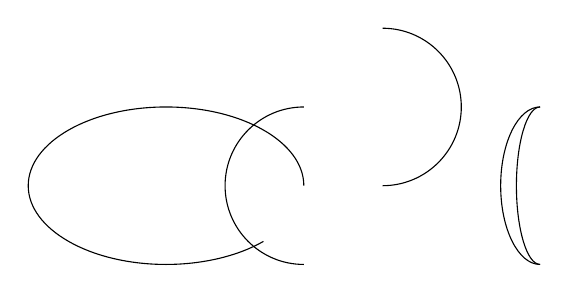
\begin{tikzpicture}
    \draw (0,1) arc (90:270:1);
    \draw (1,0) arc (-90:90:1);
    \draw (3,1) arc (90:270:0.3 and 1);
    \draw (3,1) arc (90:270:0.5 and 1);
    \draw (0,0) arc (0:315:1.75cm and 1cm);
\end{tikzpicture}


%%%%%%%%%%%%%%%%%%%%%%%%
\subsubsection{Arrow}
To draw the arrow head whthin the line, use \emph{decorate} option. \\
(need \verb|\usetikzlibrary{decorations.markings}|)


\begin{tikzpicture}
    \tikzstyle arrowstyle=[scale=1]
    \tikzstyle directed=[postaction={decorate,decoration={markings,
    mark=at position .65 with {\arrow[arrowstyle]{stealth}}}}]
    \tikzstyle reversed directed=[postaction={decorate, decoration={markings,
    mark=at position .65 with {\arrowreversed[arrowstyle]{stealth}}}}]

    \draw [red, ultra thick, directed] (0,0) -- (2,2);
\end{tikzpicture}

%%%%%%%%%%%%%%%%%%%%%%%%
\subsubsection{control points}
Control points in drawing.

\hfill
\begin{tikzpicture}
    \fill[GreenYellow!35] (-5pt, -5pt) rectangle (2cm+5pt, 2cm+5pt);

    \filldraw [gray] (0,0) circle (2pt)
		     (1,1) circle (2pt)
		     (2,1) circle (2pt)
		     (2,0) circle (2pt);
    \draw (0,0) .. controls (1,1) and (2,1) .. (2,0);

    \footnotesize
    \draw[shift={(2,1)}, xshift=0.5cm]
    node [right, text width=12cm, rounded corners, fill=blue!20,inner sep=1ex]
    {
	\begin{lstlisting}[language=TeX]
\begin{tikzpicture}
    \filldraw [gray] (0,0) circle (2pt)
		     (1,1) circle (2pt)
		     (2,1) circle (2pt)
		     (2,0) circle (2pt);
    \draw (0,0) .. controls (1,1) and (2,1) .. (2,0);
\end{tikzpicture}
	\end{lstlisting}
    };
\end{tikzpicture}

\hfill
\begin{tikzpicture}
    \fill[GreenYellow!35] (-1.5cm-5pt, -1.5cm-5pt) rectangle (1.5cm+5pt, 1.5cm+5pt);

    \draw (-1.5,0) -- (1.5,0);
    \draw (0,-1.5) -- (0,1.5);
    \draw (-1,0) .. controls (-1,0.555) and (-0.555,1) .. (0,1)
		 .. controls (0.555,1) and (1,0.555) .. (1,0);

    \footnotesize
    \draw[shift={(1.5,0)}, xshift=0.5cm]
    node [right, text width=12cm, rounded corners, fill=blue!20,inner sep=1ex]
    {
	\begin{lstlisting}[language=TeX]
\begin{tikzpicture}
    \draw (-1.5,0) -- (1.5,0);
    \draw (0,-1.5) -- (0,1.5);
    \draw (-1,0) .. controls (-1,0.555) and (-0.555,1) .. (0,1)
		 .. controls (0.555,1) and (1,0.555) .. (1,0);
\end{tikzpicture}
	\end{lstlisting}
    };
\end{tikzpicture}

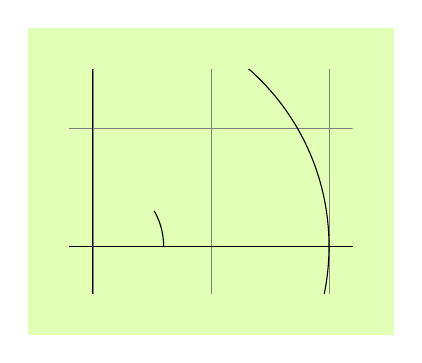
\begin{tikzpicture}[scale=3]
    \fill[GreenYellow!35] (-.1cm-5pt, -.2cm-5pt) rectangle (1.1cm+5pt, 0.75cm+5pt);

    \clip (-0.1,-0.2) rectangle (1.1,0.75);
    \draw[step=.5cm,gray,very thin] (-1.4,-1.4) grid (1.4,1.4);
    \draw (-1.5,0) -- (1.5,0);
    \draw (0,-1.5) -- (0,1.5);
    \draw (0,0) circle (1cm);
    \draw (3mm,0mm) arc (0:30:3mm);
\end{tikzpicture}

If you use relative control points, then the first one is relative to the
start node, while the second one is relative to the end node.

%%%%%%%%%%%%%%%%%%%%%%%%
\subsubsection{shade}
\verb|\shade| and \verb|\shadedraw|

\tikz \shade (0,0) rectangle (2,1)  (3,0.5) circle (0.5cm);

The default shading is a smooth transition from gray to white. To use 
other colors, specify them in options:

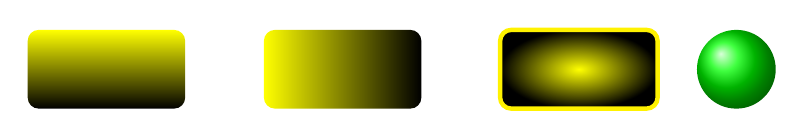
\begin{tikzpicture}[rounded corners, ultra thick]
    \shade [top color=yellow, bottom color=black] (0,0) rectangle +(2,1);
    \shade [left color=yellow, right color=black] (3,0) rectangle +(2,1);
    \shade [inner color=yellow, outer color=black, draw=yellow] (6,0) rectangle +(2,1);
    \shade [ball color=green] (9,.5) circle (0.5cm);
\end{tikzpicture}

%%%%%%%%%%%%%%%%%%%%%%%%
\subsubsection{+ sign}
\verb|+(1cm,0cm)| means ``1cm upwards from the previous specified position"; 
while \verb|++(0cm,2cm)| means ``2cm to the right of the previous specified
position, making this the {\bf new} specified position."

\tcbset{colback=brown!30}
\begin{tcolorbox}[width=4cm]
    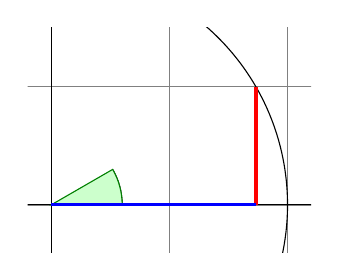
\begin{tikzpicture}[scale=3]
	\clip (-0.1,-0.2) rectangle (1.1,0.75);
	\draw[step=.5cm,gray,very thin] (-1.4,-1.4) grid (1.4,1.4);
	\draw (-1.5,0) -- (1.5,0);
	\draw (0,-1.5) -- (0,1.5);
	\draw (0,0) circle (1cm);
	\draw (3mm,0mm) arc (0:30:3mm);
	\filldraw[fill=green!20,draw=green!50!black] (0,0) -- (3mm,0mm) arc (0:30:3mm) -- cycle;
	\draw[red,very thick] (30:1cm) -- +(0,-0.5);
	\draw[blue,very thick] (30:1cm) ++(0,-0.5) -- (0,0);
\end{tikzpicture}
\end{tcolorbox}

Note the difference between \verb|+| and \verb|++| (see the code).

Using \verb|++|:

\begin{tikzpicture}
    \def\rectanglepath{-- ++(1,0) -- ++(0,1) -- ++(-1,0) -- cycle}
    \draw (0,0) \rectanglepath;
    \draw (1.5,0) \rectanglepath;
\end{tikzpicture}

Using \verb|+|:

\begin{tikzpicture}
    \def\rectanglepath{-- +(1,0) -- +(1,1) -- +(0,1) -- cycle}
    \draw (0,0) \rectanglepath;
    \draw (1.5,0) \rectanglepath;
\end{tikzpicture}

%%%%%%%%%%%%%%%%%%%%%%%%
\subsubsection{Intersection}
\verb/(<p> |- <q>)/ is ``the intersection of a vertical line through p and a horizontal line through q."

An intersection between a line going up from (1,0) and aline going from 
the origin throught (30:1cm).

\tcbset{colback=blue!20}
\begin{tcolorbox}
    \verb|\draw[very thick,orange] (1,0) -- (intersection of 1,0--1,1 and 0,0--30:1cm);|
\end{tcolorbox}

%%%%%%%%%%%%%%%%%%%%%%%%
\subsubsection{Miscellaneous}

\begin{tikzpicture}[line width=5pt]
    \draw (0,0) -- (1,0) -- (1,1) -- (0,0);
    \draw (2,0) -- (3,0) -- (3,1) -- cycle;
    \useasboundingbox (0,1.5);
\end{tikzpicture}
%%%%%%%%%%%%%%%%%%%%%%%%%%%%%%%%%%%%%%%%%%%%%%%%
\subsection{Coordinate Systems}
\begin{itemize}
    \item canvas
    \item xyz
    \item canvas polar
    \item xyz polar
    \item barycentric
	\[
	    {\alpha_1\vec{v}_1 + \alpha_2\vec{v}_2 + \cdots + \alpha_n\vec{v}_n} \over {\alpha_1 + \alpha_2 + \cdots + \alpha_n}
	    \]
    \item node
    \item intersection
    \item perpendicular
\end{itemize}
Any {\bf canvas} coordinate system requires explict dimensions (units)
while {\bf xyz} coordinate systems don't.

e.g.

\hfill
\begin{tikzpicture}
    \fill[GreenYellow!40] (-5pt,-5pt) rectangle (2cm + 5pt, 2cm + 5pt);

    \draw [help lines] (0,0) grid (2,2);

    \draw (0,0) -- (canvas polar cs:angle=30,radius=1cm);
    \draw (0,0) -- (xyz polar cs:angle=60, radius=1);

    \footnotesize
    \draw[shift={(2,1)},xshift=0.5cm]
    node [right, text width=12cm, rounded corners, fill=blue!20,inner sep=1ex]
    {
	\begin{lstlisting}[language=TeX]
\begin{tikzpicture}
  \draw [help lines] (0,0) grid (2,2);
  
  \draw (0,0) -- (canvas polar cs:angle=30,radius=1cm);
  \draw (0,0) -- (xyz polar cs:angle=60, radius=1);
\end{tikzpicture}
	\end{lstlisting}
    };
\end{tikzpicture}

\subsection{Options}
%%%%%%%%%%%%%%%%%%%%%%%%
\subsubsection{line width}
\tikz\draw[line width=2mm] (0,0)--(4,0);
\subsubsection{rotate}
\tikz\draw[rotate=45] (0,0) ellipse (16pt and 20pt);
\subsubsection{scale}
\tikz\draw[scale=1.5,rotate=75] (0,0) ellipse (10pt and 16pt);
\subsubsection{xscale, yscale}
\tikz\draw[xscale=1.5, yscale=0.5] (0,0) ellipse (10pt and 16pt);


%%%%%%%%%%%%%%%%%%%%%%%%%%%%%%%%%%%%%%%%%%%%%%%%
\subsection{node}
\tikz\draw(1,1) node{A} -- (2,2) node{B};
\hfill
\tikz\draw(1,1) node[circle, draw]{A} -- (2,2) node[circle,draw]{B};

%%%%%%%%%%%%%%%%%%%%%%%%
\subsubsection{label and pin}
\tikz[label distance=2mm]
\node[circle,fill=gray!45,label=above:12,label=right:3,label=below:6,label=left:9]{clock};
\hfill
\tikz[pin distance=4mm]\draw(1,1)
node[circle,fill=gray!45,pin=above:12,pin=right:3,pin=below:6,pin=left:9]{}
circle (1cm);

%%%%%%%%%%%%%%%%%%%%%%%%%%%%%%%%%%%%%%%%%%%%%%%%
\subsection{Styles}
tikzstyle:
\begin{itemize}
    \item every path
    \item every node
	\begin{itemize}
	    \item every \textless {\it shape} \textgreater node
	    \item every \textless {\it part name} \textgreater node part
	    \item every label
	    \item every pin
	    \item every pin edge
	\end{itemize}
    \item every to
    \item every curve
    \item every line
    \item every edge
    \item every snake
    \item every matrix
	\begin{itemize}
	    \item every cell
	\end{itemize}
    \item tree
	\begin{itemize}
	    \item every child
	    \item every child node
	    \item level \textless {\it number} \textgreater
	\end{itemize}
    \item every plot
\end{itemize}
When defining tikzstyle, there is no space allowed between the defined style and the definition.

\verb|\tikzstyle arrowstyle=[scale=1]|	\textbf{Corrected}. \\
\verb|\tikzstyle arrowstyle = [scale=1]|\textit{Wrong}.
%%%%%%%%%%%%%%%%%%%%%%%%%%%%%%%%%%%%%%%%%%%%%%%%
\subsection{plot}
%%%%%%%%%%%%%%%%%%%%%%%%
\subsubsection{gnuplot}
Tikz use \emph{gnuplot} to plot function, so to get right plot, we need to
install \emph{gnuplot} firstly. After first complining, we will get a
*.x.gnuplot file, run \emph{gnuplot} against this file, then compile tex
file again, we will get wanted plots.

difference between \verb|--plot| and \verb|plot|
\tikz\draw(0,1) -- (1,1) --plot coordinates {(2,0) (2, 1.5)};
\tikz\draw(0,1) -- (1,1) plot coordinates {(2,0) (2, 1.5)};

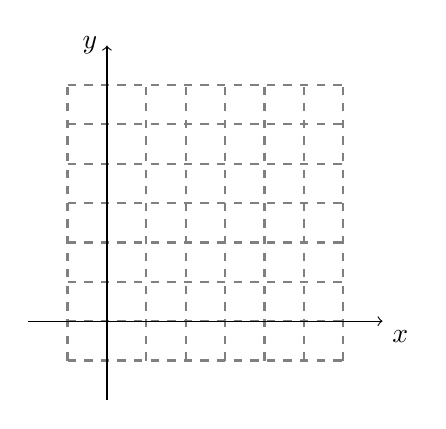
\begin{tikzpicture}[domain=0:2]
    \draw[thick,color=gray,step=0.5cm,dashed] (-0.5,-0.5) grid(3,3);
    \draw[->] (-1,0) -- (3.5,0) node[below right] {$x$};
    \draw[->] (0,-1) -- (0,3.5) node[left] {$y$};
    \draw plot[id=x] function{x*x};
\end{tikzpicture}

%%%%%%%%%%%%%%%%%%%%%%%%
\subsubsection{note on plots}
\begin{tikzpicture}
\node [anchor=west] (note) at (-1,3) {\Large Note};
\node [anchor=west] (water) at (-1,1) {\Large Water};
\begin{scope}[xshift=1.5cm]
    \node[anchor=south west,inner sep=0] (image) at (0,0)
    {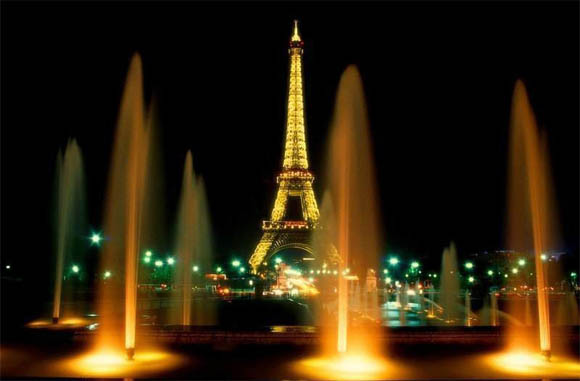
\includegraphics[width=0.7\textwidth]{eiffel.jpg}};
    \begin{scope}[x={(image.south east)},y={(image.north west)}]
        \draw[red,ultra thick,rounded corners] (0.48,0.80) rectangle (0.55,0.95);
        \draw [-latex, ultra thick, red] (note) to[out=0, in=-120] (0.48,0.80);
        \draw [-stealth, line width=5pt, cyan] (water) -- ++(0.4,0.0);
    \end{scope}
\end{scope}
\end{tikzpicture}

%%%%%%%%%%%%%%%%%%%%%%%%%%%%%%%%%%%%%%%%%%%%%%%%%%%%%%%%%%%%%%%%%%%%%%%%
\section{Examples}
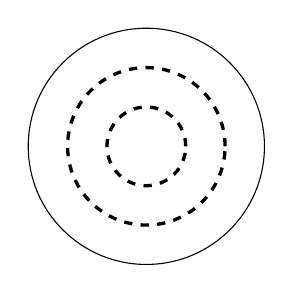
\begin{tikzpicture}
    \begin{scope}[very thick,dashed]
	\draw (0,0) circle (.5cm);
	\draw (0,0) circle (1cm);
    \end{scope}
    \draw[thin] (0,0) circle (1.5cm);
\end{tikzpicture}
\hfill

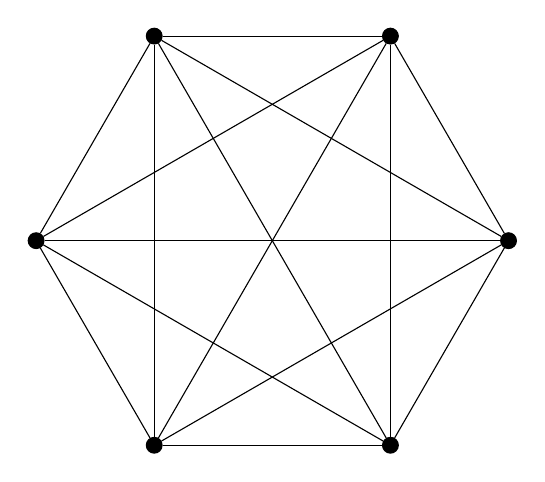
\begin{tikzpicture}[scale=1]
    \pgfmathsetmacro{\minsize}{0.2cm}
    \pgfmathsetmacro{\nodedist}{3}  
    \newcommand{\fillcolor}{black}

    \tikzstyle{every node}=[draw,shape=circle,minimum size=\minsize,inner sep=0]
    \foreach \x in {0,...,5}
	\node[fill=\fillcolor] (p\x) at (\x*60:\nodedist) {};	% (angle:radius)
    \foreach \x in {0,...,4}
    {
	\pgfmathtruncatemacro{\startvalue}{\x+1}
	\foreach \y in {\startvalue,...,5}
	    \draw (p\x) -- (p\y);
    }
\end{tikzpicture}
\hfill

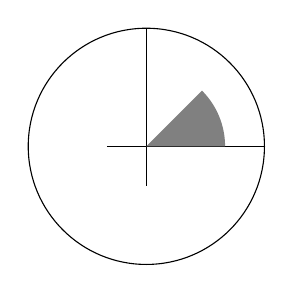
\begin{tikzpicture}
    \draw (-.5, 0)--(1.5,0);
    \draw (0, -.5)--(0, 1.5);
    \fill[gray] (0,0)--(1,0) arc (0:45:1cm) -- cycle;
    \draw[thin] (0,0) circle (1.5cm);
\end{tikzpicture}

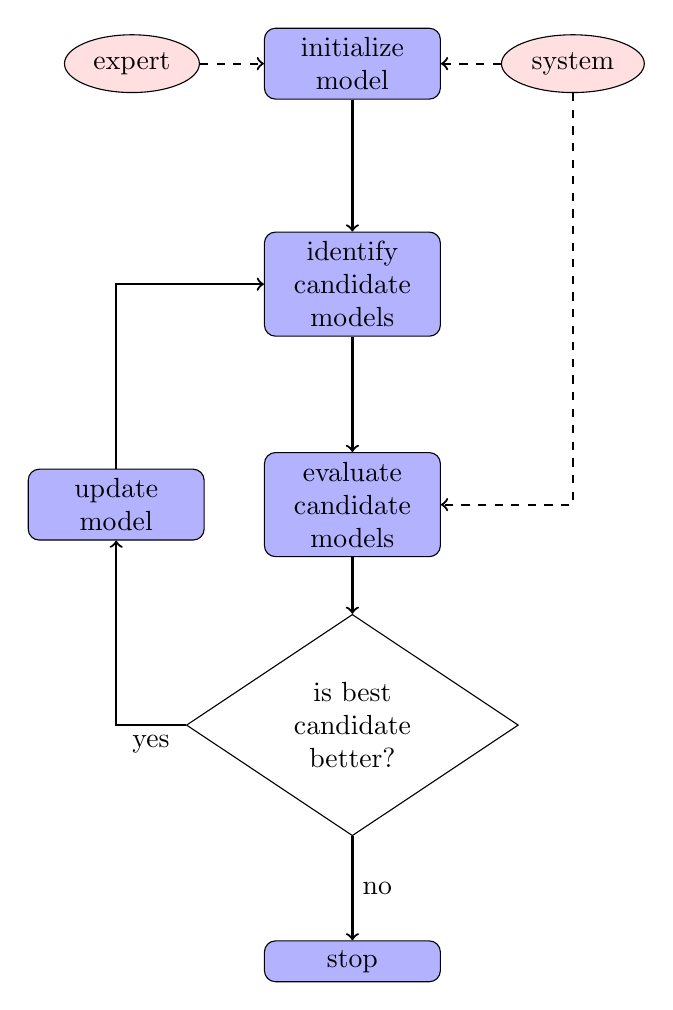
\begin{tikzpicture}[node distance=2.8cm, auto]
    \tikzstyle{block}=[rectangle, draw, rounded corners, text width=2cm,
    text centered, fill=blue!30];
    \tikzstyle{cloud}=[ellipse, draw, fill=pink!50, text centered];
    \tikzstyle{decision}=[diamond, draw,aspect=1.5,text width=2cm,text centered];
    \tikzstyle{line}=[->,black,thick,draw];
    % Place nodes
    \node [block] (init) {initialize model};
    \node [cloud, left of=init] (expert) {expert};
    \node [cloud, right of=init] (system) {system};
    \node [block, below of=init] (identify) {identify candidate models};
    \node [block, below of=identify] (evaluate) {evaluate candidate models};
    \node [block, left of=evaluate, node distance=3cm] (update) {update model};
    \node [decision, below of=evaluate] (decide) {is best candidate better?};
    \node [block, below of=decide, node distance=3cm] (stop) {stop};
    % Draw edges
    \path [line] (init) -- (identify);
    \path [line] (identify) -- (evaluate);
    \path [line] (evaluate) -- (decide);
    \path [line] (decide) -| node [near start] {yes} (update);
    \path [line] (update) |- (identify);
    \path [line] (decide) -- node {no}(stop);
    \path [line,dashed] (expert) -- (init);
    \path [line,dashed] (system) -- (init);
    \path [line,dashed] (system) |- (evaluate);
\end{tikzpicture}

\chapter{Customization}

%%%%%%%%%%%%%%%%%%%%%%%%%%%%%%%%%%%%%%%%%%%%%%%%%%%%%%%%%%%%%%%%%%%%%%%%
\section{Renewcommand}
You can modify default command by the command \verb|\renewcommand| to make
it fit your personal situation.
\begin{lstlisting}[language=TeX]
\renewcommand{\abstractname}{Executive Summary}	% Modify the title of your abstract
\renewcommand{\labelitemi}{$\triangleright$}
\renewcommand{\labelitemii}{\ding{43}}
\renewcommand{\labelitemiii}{\ding{44}}
\renewcommand{\labelitemiv}{\ding{45}}
\end{lstlisting}

%%%%%%%%%%%%%%%%%%%%%%%%%%%%%%%%%%%%%%%%%%%%%%%%
\subsection{Configuration}

%%%%%%%%%%%%%%%%%%%%%%%%
\subsubsection{Color}
\begin{lstlisting}[language=TeX]
\pagecolor[green!50!black!30]	% set page bg color
\end{lstlisting}
\subsubsection{Length}
\begin{lstlisting}[language=TeX]
\setlength{\paperwidth}{48in} 
\setlength{\paperheight}{36in}
\setlength{\sepwid}{0.024\paperwidth} % Separation width (white space) between columns
\setlength{\onecolwid}{0.22\paperwidth} % Width of one column
\setlength{\twocolwid}{0.464\paperwidth} % Width of two columns
\setlength{\threecolwid}{0.708\paperwidth} % Width of three columns
\setlength{\topmargin}{-0.5in} % Reduce the top margin size
\addtolength{\voffset}{-2.5cm}
\end{lstlisting}

%%%%%%%%%%%%%%%%%%%%%%%%%%%%%%%%%%%%%%%%%%%%%%%%%%%%%%%%%%%%%%%%%%%%%%%%
\section{New Command}
\begin{lstlisting}[language=TeX]
\newcommand{\SB}{Stony Brook}
\end{lstlisting}
Note that if type only \verb|\SB|, then the macro will eat up the following
space, producing ugly layout. To avoid that, you have to invoke it with an
empty statement after it: \verb|\SB{}|. 

The reason behind this is that \LaTeX ignores space directly after the
macro(which just stop the scanning for the macro's name). You need to break
that using either a protected space \verb|\SB\ | or an empty statement
\{\}.An empty statement is recommanded, as using a protected space can
generate nasty effects -- for example, if that protected space is directly
followed by a line break. In that case \LaTeX might pring two spaces
instead. Using an empty statement prevents this.

\verb|\def| command in {\bf plain \TeX{}} also do the work.
\begin{lstlisting}[language=TeX]
\def\intwrtx#1{\int_{-\infty}^{+\infty} #1 \,dx}
\end{lstlisting}
\def\intwrtx#1{\int_{-\infty}^{+\infty} #1 \,dx}
e.g.
$$ \intwrtx{f(x)}.$$

%%%%%%%%%%%%%%%%%%%%%%%%%%%%%%%%%%%%%%%%%%%%%%%%
\subsection{New Length}
\begin{lstlisting}[language=TeX]
\newlength{\onecolwid}{10cm}
\end{lstlisting}

or 

\begin{lstlisting}[language=TeX]
\newlength{\onecolwid}
\setlength{\onecolwid}{10cm}
\end{lstlisting}
%%%%%%%%%%%%%%%%%%%%%%%%%%%%%%%%%%%%%%%%%%%%%%%%
\subsection{New count}
\begin{lstlisting}[language=TeX]
\newcount{\opaqueness}
\end{lstlisting}

%%%%%%%%%%%%%%%%%%%%%%%%%%%%%%%%%%%%%%%%%%%%%%%%
\subsection{New dimension}
\begin{lstlisting}[language=TeX]
\newdimen{\offset}
\end{lstlisting}

%%%%%%%%%%%%%%%%%%%%%%%%%%%%%%%%%%%%%%%%%%%%%%%%%%%%%%%%%%%%%%%%%%%%%%%%
\section{Color}
\begin{lstlisting}[language=TeX]
\definecolor{mygreen}{rgb}{0,0.6,0}
\definecolor{mygray}{rgb}{0.5,0.5,0.5}
\definecolor{mypurple}{rgb}{0.58, 0, 0.82}
\end{lstlisting}

\subsection{xcolor}
\begin{lstlisting}[language=TeX]
\colorlet{LightRubinRed}{RubineRed!70!}	% xcolor; 70% or the intersity of 
% original RubineRed color. Or you can think of it as a mixture of 70% RubineRed
% and 30% white.
\colorlet{mycolor1}{green!10!orange!90!}
\definecolor{mycolor2}{HTML}{00F9DE}	% HTML model, the character A,B,C,D,E and F must be upper-case.
\end{lstlisting}

The color models that only \textbf{xcolor} support are:
\begin{itemize}
    \item \textbf{cmy} cyan, magenta, yellow
    \item \textbf{hsb} hue, saturation, brightness
    \item \textbf{HTML} RRGGBB
    \item \textbf{Gray} Grey scale, a number between 1 and 15.
    \item \textbf{wave} Wave length. Between 363 and 814    	
\end{itemize}

\chapter{Advanced}
\label{chap:Advanced}

%%%%%%%%%%%%%%%%%%%%%%%%%%%%%%%%%%%%%%%%%%%%%%%%%%%%%%%%%%%%%%%%%%%%%%%%
\section{Style}

%%%%%%%%%%%%%%%%%%%%%%%%%%%%%%%%%%%%%%%%%%%%%%%%
\subsection{Page Numbers}
How to change the numbering of pages:
\begin{lstlisting}{language=TeX}
\seccounter[page]{123}
\end{lstlisting}

How to remove all page numbers:
\begin{lstlisting}{language=TeX}
\pagestyle{empty}[page]{123}
\end{lstlisting}

\subsection{Citation}
How do I choose the square bracket or superscript style for citations:

%%%%%%%%%%%%%%%%%%%%%%%%%%%%%%%%%%%%%%%%%%%%%%%%
\subsection{Fonts}
\begin{lstlisting}[language=TeX]
\setmainfont{Times New Roman}	% serif fonts, for latin alphabetics
\setsansfont{helverica}	% latin non-serif alphabetics, usually for titles
\setmonofont{courier}	% same-width fonts, usually for code layout

% Chinese corresponding
\setCJKmainfont{simsun}
\setCJKsansfont{}
\setCJKmonofont{}   

% example: Linux Libertine
\setmainfont{LinLibertine\_R.otf}[
    BoldFont	= LinLibertine\_RZ.otf,
    ItalicFont	= LinLibertine\_RI.otf,
    BoldItalicFont = LinLibertine\_RZI.otf,
]
% sans-serif: Linux Biolinum
\setsansfont{LinLibertine\_R.otf}[
    BoldFont	= LinBiolimum\_RB.otf,
    ItalicFont	= LinBiolimum\_RI.otf,
    BoldItalicFont = LinBiolimum\_RBO.otf,
]
% typewriter type: Linux Libertine Mono
\setmonofont{LinLibertine\_M.otf}[
    BoldFont	= LinBiolimum\_MB.otf,
    ItalicFont	= LinBiolimum\_MI.otf,
    BoldItalicFont = LinBiolimum\_MBO.otf,
]

\setCJKmainfont[
    BoldFont	= Source Han Sans CN Medium,
    ItalicFont	= Adobe Kaiti Std R]
{Source Han Sans CN Light}
\setCJKsansfont[    % same as main
    BoldFont	= Source Han Sans CN Medium,
    ItalicFont	= Adobe Kaiti Std R]
{Source Han Sans CN Light}
\setCJKmonofont[
    BoldFont	= Source Han Sans CN Medium,
    ItalicFont	= Adobe Kaiti Std R]
{Source Han Sans CN Light}
\end{lstlisting}

%%%%%%%%%%%%%%%%%%%%%%%%%%%%%%%%%%%%%%%%%%%%%%%%%%%%%%%%%%%%%%%%%%%%%%%%
\section{Mode}
Using mode in \LaTeX{} allow one to choose different document class in one
tex file, for example:
\begin{lstlisting}[language=TeX]
\mode<presentation>{
    some preamble...
}

\mode<article>{
    preamble for article ...
}
\end{lstlisting}
Then if you compile a tex file (use the above one as input), then if the
documentclass is \textbf{beamer}, then mode \textbf{presentation} will be
used; if the documentclass is \textit{article}, then mode \textit{article}
will be choosed.

%%%%%%%%%%%%%%%%%%%%%%%%%%%%%%%%%%%%%%%%%%%%%%%%%%%%%%%%%%%%%%%%%%%%%%%%
\section{Adding note using tikz}
\newcommand{\annmark}[1]{%
    \textcolor{red}{$\langle$#1$\rangle$}%
}%

\newcommand{\ann}[1]{%
    \begin{tikzpicture}[remember picture, baseline=-0.75ex]%
        \node[coordinate] (inText) {};%
    \end{tikzpicture}%
    \marginpar{%
        \renewcommand{\baselinestretch}{1.0}%
        \begin{tikzpicture}[remember picture]%
            \definecolor{orange}{rgb}{1,0.5,0}%
            \draw node[fill=red!20,rounded corners,text width=\marginparwidth] (inNote){\footnotesize#1};%
    \end{tikzpicture}%
    }%
    \begin{tikzpicture}[remember picture, overlay]%
        \draw[draw = orange, thick]
            ([yshift=-0.2cm] inText)
                -| ([xshift=-0.2cm] inNote.west)
                -| (inNote.west);%
    \end{tikzpicture}%
}%

\setlength{\marginparwidth}{2.5cm}
\renewcommand{\baselinestretch}{1.3}

Freshness is the most important property for food \annmark{of course not 
for dry product }. And a good cooker will always keep food's freshness
and even enlarge the freshness using all kinds of methods.\ann{If one try to use spicy to hide all other flavor, then he must not a top cooker.} If you don't know how to cook a food, then the most obvious and simplest way is to boil it with water, which will sustain most of its freshness.

\chapter{Fantacy in \LaTeX{}}

\section{Display}
When you find something abnormal about mathmetics (wrong color), check that
if there is blank \$\$ pair without anything in it.

%%%%%%%%%%%%%%%%%%%%%%%%%%%%%%%%%%%%%%%%%%%%%%%%%%%%%%%%%%%%%%%%%%%%%%%%
\section{Package}
Updating package, if you update your texlive, and then encounter some errors
that you never met before, then it is the problem of old-packages. Remember 
to update corresponding packages so that everything work properly. Especially
when you install a new system and a new texlive but import old personal configuration.

%%%%%%%%%%%%%%%%%%%%%%%%%%%%%%%%%%%%%%%%%%%%%%%%
In \LaTeX, you can load a package many times, but the option list of each 
package loading must be a subset of the options given at the first loading (exception
\package{fontenc})

However sometimes packages might be loaded in the document class already, or
there are constraints in the package order that prevents the reordering of the 
packages. Then \command|\PassOptionsToPackage| helps. It can even
be loaded before \command|\documentclass|. It gives the specified 
options to the package without loading the package.

Adding the options to the global options can also be a solution, but it is not the
best strategy, because also other unrelated packages see that options. Unknown global 
options are ignored by package, but known are then executed with unintended side effects.

\subsection{physics \& imakeidx}
If I put package imakeidx before physics, then the compiler will complain
something like this:
\begin{verbatim}
(/usr/share/texlive/texmf-dist/tex/latex/imakeidx/imakeidx.sty
(/usr/share/texlive/texmf-dist/tex/latex/xkeyval/xkeyval.sty
(/usr/share/texlive/texmf-dist/tex/generic/xkeyval/xkeyval.tex
(/usr/share/texlive/texmf-dist/tex/generic/xkeyval/xkvutils.tex)))
(/usr/share/texlive/texmf-dist/tex/latex/tools/multicol.sty))
(/home/weibin/texmf/tex/latex/physics/physics.sty
(/home/weibin/texmf/tex/latex/l3packages/xparse/xparse.sty
(/home/weibin/texmf/tex/latex/l3kernel/expl3.sty
(/home/weibin/texmf/tex/latex/l3kernel/expl3-code.tex
! Missing number, treated as zero.
<to be read again> 
                   \pdftex_shellescape:D 
l.23338	    }
\end{verbatim}
But if I put physics before imakeidx, then no error happen.

%%%%%%%%%%%%%%%%%%%%%%%%%%%%%%%%%%%%%%%%%%%%%%%%
\subsection{tikz \& graphicx}
It looks like \textbf{tika} package will load \emph{graphicx} package
automatically, so if you load \emph{graphicx} package manually with some
options, it will cause problem. For example, if I load them as
\begin{verbatim}
\usepackage[dvips]{graphicx}
\usepackage{tikz}
\end{verbatim}
it will result in:
\begin{verbatim}
Non-PDF special ignored!
\end{verbatim}
On the other hand, if I load them as:
\begin{verbatim}
\usepackage{tikz}
\usepackage[dvips]{graphicx}
\end{verbatim}
We get such error:
\begin{verbatim}
! LaTeX Error: Option clash for package graphicx.
\end{verbatim}

So this should be the conflicts between different options used in loading
\emph{graphicx} package. If you load only the \textbf{tikz} package, 
then everything works perfectly.

% graphics
! Paragraph ended before \\Gin@iii was complete.    \\
You will encounter this error if you load \emph{graphics} rather than \emph{graphicx}.
%%%%%%%%%%%%%%%%%%%%%%%%%%%%%%%%%%%%%%%%%%%%%%%%
\subsection{xcolor}
\package{xcolor} option error:
\begin{verbatim}
! LaTeX Error: Option clash for package xcolor.
\end{verbatim}
Package \package{pgf} also load \package{xcolor}, so
\package{xcolor} should be loaded before \package{pgf} or 
other packages that loads \package{pgf}.

%%%%%%%%%%%%%%%%%%%%%%%%%%%%%%%%%%%%%%%%%%%%%%%%%%%%%%%%%%%%%%%%%%%%%%%%
\section{Environment}

%%%%%%%%%%%%%%%%%%%%%%%%%%%%%%%%%%%%%%%%%%%%%%%%
\subsection{gathered}
No blank line allowed with \emph{gathered} environment, otherwise, it will show
error message:
\begin{verbatim}
! Missing $ inserted.
<inserted text> $
\end{verbatim}

%%%%%%%%%%%%%%%%%%%%%%%%%%%%%%%%%%%%%%%%%%%%%%%%%%%%%%%%%%%%%%%%%%%%%%%%
\section{Options}
%%%%%%%%%%%%%%%%%%%%%%%%%%%%%%%%%%%%%%%%%%%%%%%%
\subsection{aligned}
In the \emph{aligned} environment, if you begin you equation with \textbf{square bracket},
they will not be output normally, because aligned env. is set by the \emph{amsmath} package to scan ahead for a positioning augument such as [t] of [p]. Material that's found there but doesn't meet this format is simply discarded.	

The possible solutions are:
\begin{itemize}
    \item Insert \verb|\relax| before the left square bracket. It will stop the bracket from being interpreted as an argument.
    \item Insert \{\} before the left square brackedt.
\end{itemize}

%%%%%%%%%%%%%%%%%%%%%%%%%%%%%%%%%%%%%%%%%%%%%%%%%%%%%%%%%%%%%%%%%%%%%%%%
\section{order of commands}
%%%%%%%%%%%%%%%%%%%%%%%%%%%%%%%%%%%%%%%%%%%%%%%%
\subsection{label and caption}
If you put \verb|\label| command before the \verb|\cpation| command, then \verb|\ref| will not show the correct citation;
if you just exchange their place, then you get everything work well, weird.

\chapter{Bibliography}
Things about citing bibliography.

% \input{}
% \include{hello_world/Package}
\end{document}
